\chapter{Introduction}
\label{cha:introduction}


\paragraph{}
This project was conducted following five steps. Firstly, by analysing the historical background related to pedagogy with technologies and researching the related work. The second step was to establish a model with the ideal tool that could satisfy the goal set forth for the project. Third, define an evaluation method to justly judge and assess the efficiency of the implementation. Fourth, select a wide range of individuals that represent various classes of target users and perform the experiment and survey. And finally, draw conclusions and inferences from the resulting data to either prove the point accentuated in the Abstract section or to reevaluate and share the yielded knowledge with the academic world.

\section{Background}
\paragraph{}
As mentioned in the Abstract section, this projects sets forth with the important judgement that learning practices follow a seemingly delayed convention as to what tools and systems should be used. Modern technology adoption follows several phases or life cycles which obey the Roger's bell*. As shown statistically, academic adoption of technology generally materializes in the closing end of the wave. This phenomenon has many factors and reasons that justify the norm. For instance, if we use teachers as an example, who mostly are accustomed to follow a model, of which they have come to feel experienced with, the change to different practices and principles has a high probably to jeopardize the productivity of the teaching process. Of course the point of this dissertation is not to question the patterns of teachers and the reasons why many chose to maintain the customs they feel most confident with, but instead to simply point out, that the learning process is an exercise carried out by and for the student, who has the choice and flexibility to undertake any system of learning and should as such be exposed to a wide variety. It is my opinion that students have a predisposition to discard newer technologies for their teachers disbelief's, which might end up having the unfortunate consequence of depriving a student from a more efficient practicing system than any other they may be familiar with.

The development of a Smart Speaker as Studying Assistant sets out to defy this norm and prove that early technology adoption might boost the learning productivity, if the software is easy enough to use. The Studying Assistant skill developed for the Alexa devices follows no bleeding edge theories on efficient pedagogy, but merely simplifies the process to repeat and replicate a practicing dialog of asking and answering simple multiply choice questions, specially in parallel with any other activities that might not disrupt the oral communication with the device.

This project is focused on two aspects regarding the developed tools. The first aspect argues the importance of such a tool from a pedagogical stand point. What it represents in the timeline of teaching and studying habits as well as what consequences it poses by changing these. 

The second is more centered on the adoption of new technologies in general, what approaches and measures should be taken to either append to one user's practices, the attitude and mindset towards technology in general and the specific tool, or to replace already established ones, perceived ease of use.



\begin{itemize}
	\item{Bullet point 1}
	\item {Bullet point 2}
\end{itemize}


\section{New Section}

New Section........is shown in Figure \ref{fig:eduTec}........

\begin{figure}[h]
	\centering
	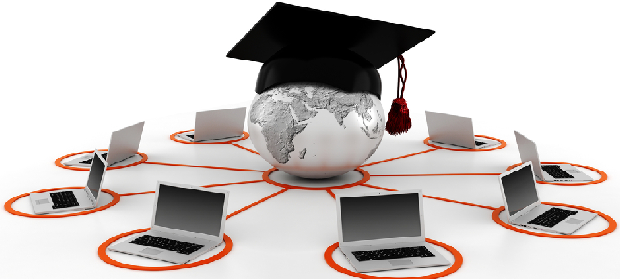
\includegraphics[width=1\textwidth]{images/eduTec.png}
	\caption{Educational Technologies \cite{google}}
	\label{fig:eduTec} 
\end{figure}
\FloatBarrier

Vel ex debitis accusam interpretaris, vis te dico accommodare. Vero verear vis cu. At alterum accusamus pri, qui an praesent efficiendi. Nobis sadipscing in eum, ne cetero appareat vim. Ea vide dicit pri, et adhuc omnesque scripserit est. Quo idque oratio facete cu, mazim doctus fabellas vim an, ea fugit expetendis ius.


\section{Research Question}
The research questions related with this thesis work are: 

\begin{enumerate}
	
\item How..............?

\item What.............?

\end{enumerate}

\section{Outline}
The remaining part of the thesis is organized as follows:

In the second chapter, we discuss the related work...................

